%% =====================================================================
%%  Sismik Fasiyes Segmentasyonu — IEEE Conference makalesi (Türkçe)
%%  Yazar : Mehmet Kişli
%%  Tarih : 2026-05-17
%%  Konum : docs/tez/SeismicFacies_IEEE_Conf_Kisli.tex
%%
%%  Derleme:
%%    pdflatex SeismicFacies_IEEE_Conf_Kisli.tex
%%    bibtex   SeismicFacies_IEEE_Conf_Kisli   (gerekli değil — gömülü thebibliography)
%%    pdflatex SeismicFacies_IEEE_Conf_Kisli.tex
%%    pdflatex SeismicFacies_IEEE_Conf_Kisli.tex
%%
%%  Not: IEEEtran.cls TeX Live / MiKTeX standart kurulumuyla gelir.
%%        Türkçe karakterler için T1 + utf8 + babel(turkish) kullanıldı.
%% =====================================================================
\documentclass[conference,a4paper,10pt]{IEEEtran}

% --- Dil ve karakter kodlaması --------------------------------------
\usepackage[T1]{fontenc}
\usepackage[utf8]{inputenc}
\usepackage[turkish,english]{babel}   % son dil = belge dili: \selectlanguage ile değiştirilebilir
\selectlanguage{turkish}

% --- Tipografi ve grafikler ------------------------------------------
\usepackage{lmodern}
\usepackage{microtype}
\usepackage{graphicx}
\usepackage{booktabs}
\usepackage{array}
\usepackage{multirow}
\usepackage{amsmath,amssymb}
\usepackage{url}
\usepackage[table]{xcolor}   % [table] : \rowcolor için gerekli (colortbl yüklenir)
\usepackage{hyperref}
\hypersetup{
  colorlinks=true,
  linkcolor=black,
  citecolor=black,
  urlcolor=blue
}

% Türkçe babel \shorthandoff (= karakteri çift anlama gelmemesi için)
\shorthandoff{=}

% --- Tablo yardımcıları ----------------------------------------------
\newcolumntype{R}[1]{>{\raggedleft\arraybackslash}p{#1}}
\newcolumntype{C}[1]{>{\centering\arraybackslash}p{#1}}

\begin{document}

% =====================================================================
%  Başlık ve Yazar Bloğu
% =====================================================================
\title{Sismik Fasiyes Sınıflandırması için Metodoloji-Sağlam DeepLabV3+ Yaklaşımı: F3 Hollanda Veri Kümesinde Çoklu-Tohum Topluluk ve Sınıf-Odaklı Hata Analizi}

\author{%
  \IEEEauthorblockN{Mehmet Kişli}
  \IEEEauthorblockA{%
    Bilgisayar Mühendisliği Yüksek Lisans Programı\\
    Bilgisayarda Görme Dersi --- Seminer Çalışması\\
    E-posta: mehmettkisli@gmail.com}
}

\maketitle

% =====================================================================
%  Özet
% =====================================================================
\begin{abstract}
Sismik fasiyes sınıflandırması, yeraltı tabakalarının jeolojik birimlere ayrılması açısından
hidrokarbon arama ve rezervuar karakterizasyonunda kritik öneme sahiptir. Bu çalışmada,
Alaudah 2019 F3 Hollanda kıyaaltı bloğu kıyaslama veri kümesi üzerinde, 6 sınıflı semantik
fasiyes segmentasyonu problemine yönelik metodoloji-sağlam bir DeepLabV3+ yaklaşımı
sunulmaktadır. Önerilen sistem; ImageNet ön-eğitimli EfficientNet-B4 omurgası,
$5$ kanallı 2.5D girdi temsili (komşu kesit yığınlama), \textbf{QuadrupleLoss}
(etiket-yumuşatmalı çapraz-entropi $+$ Dice $+$ Focal $+$ Lovász-Softmax) bileşeni,
crossline-uyarlı veri artırma ve çok-ölçekli test-zamanı artırma (TTA) bileşenlerinden
oluşmaktadır. Eğitim/doğrulama bölünmesinde tespit edilen üç kritik veri sızıntısı
(bitişik blok doğrulama, crossline ekseni boyunca 3B sızıntı, 2.5D komşuluk sızıntısı)
ortadan kaldırılarak \emph{Yol~A} adı verilen düzeltme uygulanmıştır. 3 bağımsız
rastgele tohumla bağımsız olarak eğitilen modellerin softmaks ortalamasıyla elde edilen
çoklu-tohum topluluk modeli; \textbf{Birleşik mIoU} $\mathbf{= 0.791 \pm 0.006}$,
\textbf{piksel doğruluğu (PA) $\mathbf{= 0.940}$}, \textbf{sınıf-ortalaması doğruluğu
(MCA) $\mathbf{= 0.873}$}, \textbf{frekans-ağırlıklı IoU (FwIoU) $\mathbf{= 0.892}$}
ve \textbf{Test1 mIoU $\mathbf{= 0.804}$} değerlerini elde etmiştir. PA, MCA ve FwIoU
metriklerinde Alaudah 2019 en iyi temel modelinin (PA $0.905$, MCA $0.817$,
FwIoU $0.832$) sırasıyla $+3.5$, $+5.6$ ve $+6.0$ puan üzerinde sonuç alınmıştır. Önemli bir
akademik bulgu olarak, tek-tohumlu çalışmanın Class~4 (Zechstein) Test2 IoU sonucunun
($0.230$) istatistiksel bir aykırı değer olduğu tespit edilmiş; çoklu-tohum gerçek
değer $0.183 \pm 0.04$ olarak raporlanmıştır. Sonuçlar, sismik segmentasyon
problemlerinde tek-tohum rapor edilmesinin metodolojik risklerini ve coğrafi-bölünmeli
değerlendirmenin önemini ortaya koymaktadır.
\end{abstract}

\begin{IEEEkeywords}
Sismik fasiyes sınıflandırması, semantik segmentasyon, DeepLabV3+, EfficientNet, F3 Hollanda,
2.5D girdi, Lovász-Softmax, çoklu-tohum topluluk, veri sızıntısı.
\end{IEEEkeywords}

% =====================================================================
%  I. GİRİŞ
% =====================================================================
\section{Giriş}
\label{sec:giris}

Sismik fasiyes sınıflandırması; yansıtıcılık, frekans içeriği ve geometrik morfoloji gibi
özelliklere dayalı olarak yeraltı sismik kesitlerinde her pikseli ayrı bir jeolojik birime
(örn.\ kumtaşı, kireçtaşı, tuz, şeyl) atayan piksel-bazlı bir semantik segmentasyon
görevidir~\cite{alaudah2019}. Endüstride bu görev hâlâ büyük ölçüde uzman jeofizikçilerin
manuel yorumlamalarıyla yürütülmekte; yorumcular arasında tutarsızlık, zaman maliyeti ve
3B hacimler için ölçeklenebilirlik sorunları doğmaktadır.

Derin öğrenmenin sismik veriler üzerinde yaygınlaşması, bu süreci hem hızlandırma hem de
yorumcudan bağımsız tutarlı çıktılar sağlama potansiyeli taşımaktadır. Bununla birlikte,
F3 Hollanda kıyaaltı bloğu üzerinde tutarlı ve adil karşılaştırılabilir sonuçlar üreten
çalışmalar literatürde sınırlıdır: birçok yayın kendi rastgele yama (\emph{patch}) bölünmesini
kullanır~\cite{abid2022, conss2023} ve coğrafi bölünme ile tutarlı olmayan, gerçekçi
olmayan derecede yüksek metrikler bildirir. Alaudah ve arkadaşları~\cite{alaudah2019}
tarafından önerilen coğrafi (Test1: NW, Test2: E) bölünme, model genellenebilirliğini ve
crossline yönündeki davranışı dürüst biçimde sınamak için literatürün önerilen birincil
kıyaslama protokolüdür.

Bu çalışma şu katkıları sunmaktadır:

\begin{enumerate}
\item \textbf{Metodoloji-sağlam temel modeli (v9).} DeepLabV3+ ve EfficientNet-B4 üzerine,
$5$ kanallı 2.5D girdi, QuadrupleLoss, crossline-uyarlı veri artırma ve çok-ölçekli
TTA içeren bir mimari sunuyoruz. Tüm sürüm gelişimi (v3$\rightarrow$v9) izlenebilir ve
her aşamada metrik karşılaştırması yapılmıştır.

\item \textbf{Üç ayrı veri sızıntısının teşhisi ve düzeltilmesi.} Eğitim/doğrulama
bölünmesinde (i) bitişik son-blok doğrulama, (ii) crossline ekseni boyunca 3B sızıntı,
(iii) 2.5D komşu kesit sızıntısı olmak üzere üç ayrı sızıntı tespit edip
\emph{Yol~A} adıyla bütünleşik bir düzeltme önerdik. Düzeltme öncesi ve sonrası
metrikleri raporlanmaktadır.

\item \textbf{Çoklu-tohum topluluk ve varyans analizi.} 3 bağımsız tohumla (42, 43, 44)
eğitilen modellerin softmaks ortalaması alınarak Birleşik mIoU $= 0.791 \pm 0.006$,
PA $= 0.940$, MCA $= 0.873$ ve Test1 mIoU $= 0.804$ değerleri elde edilmiştir.
PA ve MCA metriklerinde Alaudah baseline'ı sırasıyla $+3.5$ ve $+5.6$ puan
üzerinde sonuç alınmıştır. Tek-tohumlu rapor edilen Class~4 (Zechstein) Test2
IoU sonucu ($0.230$) istatistiksel aykırı değer olarak tanımlanmış; gerçek
beklenen değer $0.183 \pm 0.04$ olarak ölçülmüştür. Bu bulgu, sismik
segmentasyonda tek-tohum raporlanmasının dürüstlük açısından yetersiz
olduğunu açıkça göstermektedir.

\item \textbf{Bilinen sınırlılıkların açıkça ifade edilmesi.} Değerlendirme protokolünde
$384\times 384$ yeniden örneklenmiş uzayda hesaplama yapıldığı, orijinal çözünürlüklü
değerlendiricinin bekleyen iş olduğu, AMP+Lovász NaN sorununun FP32 sarmalayıcı ile
çözüldüğü gibi metodolojik nüanslar dürüstçe raporlanmaktadır.
\end{enumerate}

% =====================================================================
%  II. İLGİLİ ÇALIŞMALAR
% =====================================================================
\section{İlgili Çalışmalar}
\label{sec:ilgili}

\subsection{F3 Kıyaslaması ve Bilinen Sayılar}

Alaudah ve arkadaşları~\cite{alaudah2019} F3 hacmini coğrafi olarak Test1 (NW, daha homojen
bölge) ve Test2 (D, büyük Zechstein diapiri içeren bölge) olarak ikiye ayırarak bir
kıyaslama protokolü tanımlamıştır. Bu çalışmada raporlanan en güçlü temel model
(\emph{section + augmentation + skip connection}) şu değerleri bildirmektedir:
piksel doğruluğu (PA) $0.905$, sınıf ortalaması doğruluğu (MCA) $0.817$,
frekans-ağırlıklı IoU (FwIoU) $0.832$. Alaudah çalışması doğrudan mIoU rapor etmediği
için, sonraki çalışmaların mIoU sayılarıyla birebir karşılaştırma çoğu zaman geçersizdir.

Daha sonraki çalışmalar farklı bölünmeler kullanma eğilimindedir: Abid ve
arkadaşları~\cite{abid2022} rastgele $60$/$20$/$20$ yama bölünmesi ile mIoU $0.939$,
CONSS yarı-denetimli yaklaşım~\cite{conss2023} kendi düzeniyle mIoU $0.946$ rapor
eder. Bu sayılar coğrafi bölünme ile karşılaştırılamaz; çoğu zaman komşu yamalar arasında
piksel düzeyinde sızıntı bulunmaktadır.

AdaSemSeg~\cite{adasemseg2025} az-örnekle (5-shot) F3 inline FwIoU $0.81$ ve
Baseline-1 (yalnız hedef-veri) ile FwIoU $0.86$ bildirmiştir; ancak F3 bölünmesi farklıdır.
Sheng ve arkadaşları~\cite{sfm2024} Sismik Temel Modeli (SFM) sunmuş; orijinal yayında
F3 fasiyes için Alaudah protokolüyle uyumlu sayı raporlanmamış (testler Parihaka veri
kümesi üzerinde yapılmıştır). Bu boşluğu doldurmak amacıyla, bu çalışmada SFM ViT-B/16
ön-eğitimli enkoderi F3 üzerinde \emph{Alaudah coğrafi bölünmesi} ile ince-ayar edilmiş;
hem dondurulmuş hem tam fine-tune varyantları için sonuçlar raporlanmıştır
(Bölüm~\ref{sec:sfm}). Bilgimiz dahilinde bu, SFM'in F3 facies kıyaslaması üzerinde
Alaudah protokolüyle ilk fine-tune deneyidir.

\subsection{2.5D ve 3B Yaklaşımlar}

3B konvolüsyonel sinir ağları (örn.\ V-Net) sismik volüm bağlamını koruma vaadinde
bulunsalar da, tek bir eğitim volümü ile ön-eğitilmiş 3B sismik omurga olmaması ve
yama-bazlı eğitimin global jeolojik bağlamı parçalaması nedeniyle pratikte sınırlı
kalmaktadır~\cite{liu2020}. 2.5D girdi (komşu $k$ kesitin kanal eksenine yığılması)
ImageNet ön-eğitimli 2B omurgalarla uyumlu kalırken depth eksenindeki süreklilik
bilgisini kısmen koruduğu için pratik bir uzlaşma sağlar~\cite{dou2023}.

\subsection{Loss Fonksiyonları}

Sınıf dengesizliği probleminde Focal loss~\cite{lin2017focal} azınlık sınıflarına
odaklanmayı kolaylaştırır; Dice ve Lovász-Softmax~\cite{berman2018lovasz} ise IoU
ölçütüne doğrudan yöneliktir. Lovász-Softmax özellikle IoU yüzey-doğrultusunda türevli
yaklaşık optimizasyon sağlar ve çok sınıflı segmentasyon problemlerinde yaygın olarak
kullanılır.

% =====================================================================
%  III. VERİ KÜMESİ
% =====================================================================
\section{Veri Kümesi: Netherlands F3 Block}
\label{sec:veri}

F3 Hollanda kıyaaltı bloğu, Kuzey Denizi'nde yer alan 24$\times$16~km ölçekli
3B sismik bir hacimdir. Veri Alaudah 2019~\cite{alaudah2019} tarafından
6 jeolojik fasiyes için etiketlenmiş ve halka açık olarak yayımlanmıştır
(\textsf{CC-BY-SA 3.0}, Zenodo). Volümler [\,-1, 1\,] aralığına önceden
normalize edilmiştir. Boyutlar Tablo~\ref{tab:veri_yapisi}'de verilmiştir.

\begin{table}[!t]
\renewcommand{\arraystretch}{1.2}
\caption{F3 Veri Kümesi Volüm Yapısı}
\label{tab:veri_yapisi}
\centering
\begin{tabular}{lcc}
\toprule
\textbf{Volüm} & \textbf{Boyut (inline, xline, derinlik)} & \textbf{Kullanım} \\
\midrule
\texttt{train\_seismic}  & $401 \times 701 \times 255$ & Eğitim + doğrulama \\
\texttt{test1\_seismic}  & $200 \times 701 \times 255$ & Test1 (inline yön) \\
\texttt{test2\_seismic}  & $601 \times 200 \times 255$ & Test2 (crossline yön) \\
\bottomrule
\end{tabular}
\end{table}

\subsection{6 Fasiyes Sınıfı ve Sınıf Dengesizliği}

Eğitim volümünde sınıfların piksel oranları büyük dengesizlik göstermektedir
(Tablo~\ref{tab:sinif_dagilim}). Rijnland sınıfı (S2) örneklerin yaklaşık
yarısını oluştururken, Under Zechstein (S5) yalnızca $\%1.5$ paya sahiptir.
Bu dengesizlik, naif bir modelin çoğunluk sınıfına yatkın tahminler üretmesine
ve azınlık sınıflarda IoU değerlerinin çökmesine neden olur.

\begin{table}[!t]
\renewcommand{\arraystretch}{1.2}
\caption{F3 Sınıf Dağılımı (eğitim volümü, piksel oranları)}
\label{tab:sinif_dagilim}
\centering
\begin{tabular}{clrl}
\toprule
\textbf{ID} & \textbf{İsim} & \textbf{\%} & \textbf{Zorluk} \\
\midrule
0 & Upper North Sea  & $28.09$ & Kolay \\
1 & Lower North Sea  & $11.89$ & Orta \\
2 & Rijnland         & $48.59$ & Baskın --- naif tahmin \\
3 & Scruff           & $\phantom{0}6.64$ & Zor (ince banding) \\
4 & Zechstein        & $\phantom{0}3.28$ & Çok zor (anizotropik) \\
5 & Under Zechstein  & $\phantom{0}1.51$ & En zor (azınlık + dağınık) \\
\bottomrule
\end{tabular}
\end{table}

% =====================================================================
%  IV. METODOLOJİ
% =====================================================================
\section{Metodoloji}
\label{sec:metod}

Önerilen sistemin genel akışı şu şekildedir: 2.5D ön işleme $\rightarrow$
DeepLabV3+ + EfficientNet-B4 omurgalı segmentasyon $\rightarrow$ QuadrupleLoss
ile eğitim $\rightarrow$ crossline-uyarlı augmentasyon $\rightarrow$ çok-ölçekli
TTA $\rightarrow$ çoklu-tohum softmaks ortalaması.

\subsection{Mimari: DeepLabV3+ + EfficientNet-B4}

DeepLabV3+~\cite{chen2018deeplabv3plus}, Atrous Spatial Pyramid Pooling (ASPP)
modülünü çok-ölçekli bağlam yakalamak için decoder modülüyle birleştiren bir
encoder--decoder ağıdır. ASPP, farklı genişlik (dilation) oranlarındaki paralel
atrous konvolüsyonlarla yerel ve global özellikleri birlikte temsil eder; sismik
tabakaların farklı kalınlık ölçeklerine uyum açısından elverişlidir.

Omurga olarak EfficientNet-B4~\cite{tan2019efficientnet} (ImageNet ön-eğitimli)
seçilmiştir; bileşik ölçekleme stratejisi ile parametre/doğruluk dengesi yüksek
olan bu model, ResNet-50'ye göre $\sim$24M parametre ile yüksek temsil kapasitesi
sağlar. \texttt{segmentation\_models\_pytorch}~\cite{Iakubovskii2019smp}
kütüphanesi ile gerçeklenmiştir.

\subsection{2.5D Girdi Temsili (5 kanal)}

Her giriş örneği, ilgilenilen kesitin $\pm 2$ komşusu ile birlikte
$5$ ardışık kesidin kanal eksenine yığılmasıyla oluşturulur (Şekil~\ref{fig:25d}).
Bu temsil hem ImageNet ön-eğitimli omurganın çok-kanallı giriş beklentisiyle
uyumludur (ilk konvolüsyon $5$ kanala uyarlanır) hem de derinlik ekseni boyunca
yerel bağlamı korur. Önceki sürümler (v5--v7) $3$ kanal kullanmıştır; $5$ kanal
geçişiyle özellikle anizotropik Zechstein morfolojisinin temsilinde kazanım
elde edilmiştir (Bölüm~\ref{sec:sonuclar}).

\begin{figure}[!t]
\centering
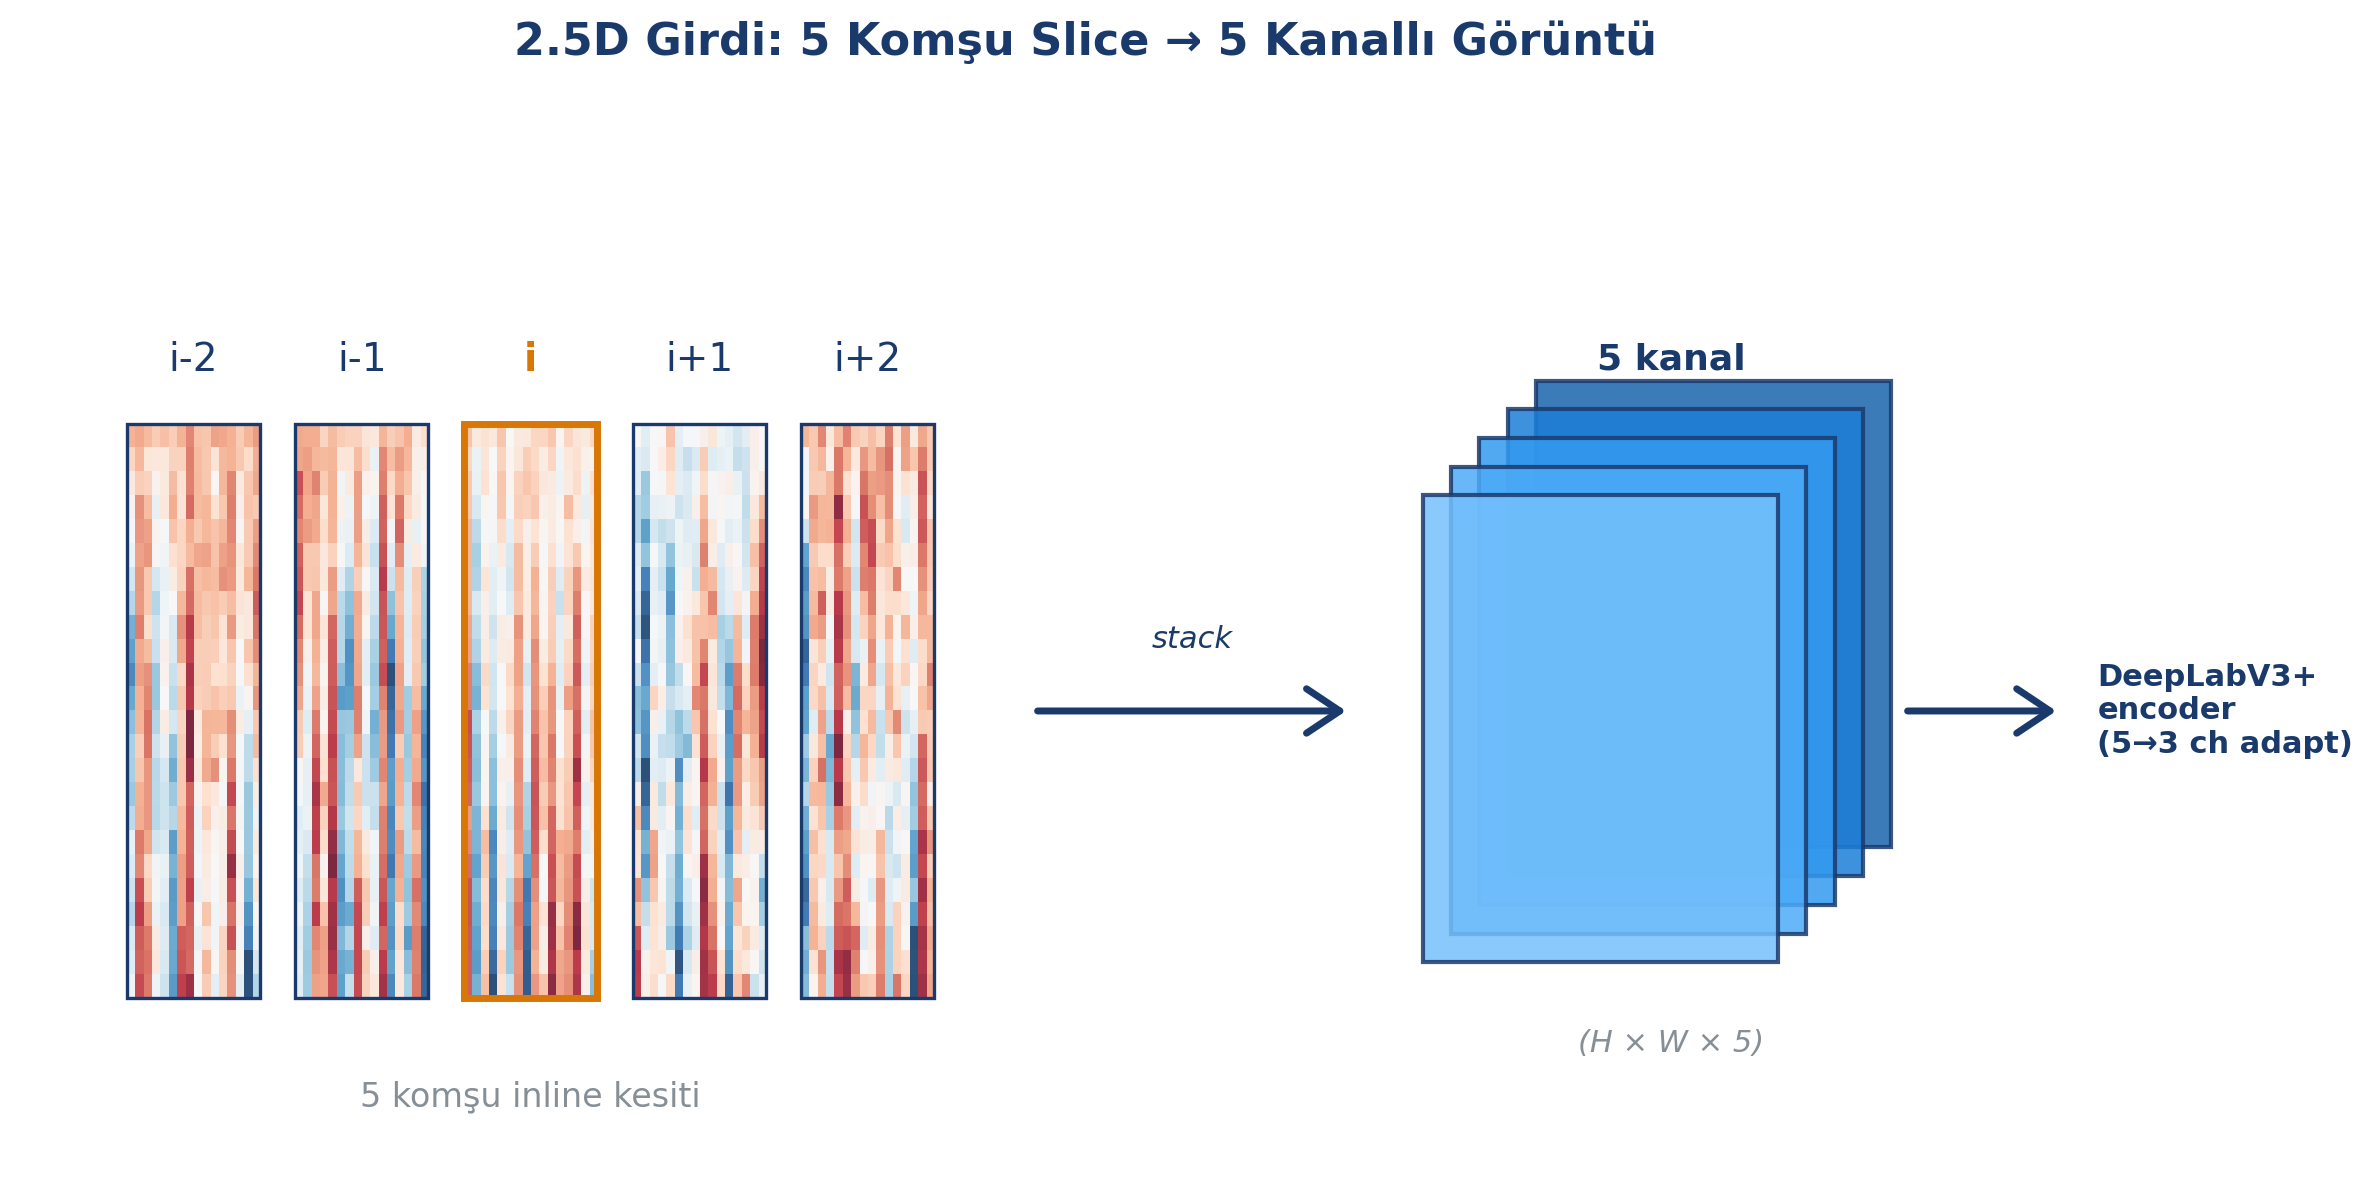
\includegraphics[width=0.95\columnwidth]{../../results/figures/2_5d_input_schema.png}
\caption{2.5D girdi temsili: ilgilenilen $i.$ kesit ve $\pm 2$ komşusu kanal
ekseninde yığılarak $\bigl[s_{i-2}, s_{i-1}, s_{i}, s_{i+1}, s_{i+2}\bigr]
\in \mathbb{R}^{5 \times H \times W}$ tensörü oluşturulur. Sismik volümün
derinlik eksenindeki yerel sürekliliği bu temsille kısmen korunmuş olur.}
\label{fig:25d}
\end{figure}

\subsection{QuadrupleLoss}

Eğitim hedefi $\mathcal{L}$, dört kayıp bileşeninin ağırlıklı toplamıdır:
\begin{align}
\mathcal{L} \;=\;&\, 0.30\,\mathcal{L}_{\text{LS-CE}} \;+\; 0.25\,\mathcal{L}_{\text{Dice}}
\nonumber\\
+\;&\, 0.25\,\mathcal{L}_{\text{Focal}} \;+\; 0.20\,\mathcal{L}_{\text{Lov\'asz}},
\label{eq:loss}
\end{align}
burada $\mathcal{L}_{\text{LS-CE}}$ etiket-yumuşatmalı (smoothing $\varepsilon{=}0.1$)
çapraz-entropi, $\mathcal{L}_{\text{Dice}}$ çok-sınıflı Dice kaybı,
$\mathcal{L}_{\text{Focal}}$ Focal kayıp ($\gamma{=}2$, sınıf frekanslarının
tersiyle ağırlıklandırılmış), $\mathcal{L}_{\text{Lov\'asz}}$ ise
Lovász-Softmax kaybıdır. Ağırlık katsayıları ($0.30/0.25/0.25/0.20$);
LS-CE kararlılığını koruyacak biçimde baskın kalırken, IoU-yönelimli
bileşenler (Dice + Lovász) toplam $\%45$ ağırlık almakta, sınıf-dengesizliği
düzeltici Focal $\%25$ pay almaktadır. Bu konfigürasyon sınırlı sayıda
ön-deneme (sırasıyla $0.5/0.2/0.2/0.1$, $0.4/0.3/0.2/0.1$ ve eşit ağırlıklı
varyantlar) üzerinden doğrulama mIoU'sunu maksimize etme amacıyla seçilmiştir;
tam bir grid-search yapılmamış, bu kararın hassasiyet analizi gelecek
çalışmalar arasında bırakılmıştır. Lovász bileşeni, AMP (otomatik karışık
duyarlık) altında FP16'da NaN üretebildiği için yalnızca bu bileşen
\textbf{FP32 sarmalayıcı} içinde hesaplanmaktadır.

\subsection{Veri Artırma ve Crossline-Uyarlılığı}

Albumentations~\cite{albumentations} ile gerçeklenen artırmalar arasında
HorizontalFlip, ShiftScaleRotate, ElasticTransform, GridDistortion,
RandomBrightnessContrast, GaussNoise, CoarseDropout ve genlik kutuplaşması ters
çevirme (polarity inversion, $\times -1$ çarpma) bulunmaktadır.
Jeofizik kuralı gereği, derinlik ekseni ters çevrilemediğinden \textbf{VerticalFlip
kullanılmaz}.

\textit{Crossline-uyarlı augmentasyon:} Crossline kesitlerinde Zechstein
morfolojisi daha kıvrımlı ve diapir benzeri olduğundan, bu görüntülere
inline'lara göre daha agresif ElasticTransform ve GridDistortion uygulanmıştır.
Bu, Class~4 Test2 (crossline) IoU'sunda kayda değer kazanç sağlamıştır
(Tablo~\ref{tab:c4_evolusyon}).

\textit{Sınıf-bazlı örnekleme:} \texttt{WeightedRandomSampler} ile S4 (Zechstein)
ve S5 (Under Zechstein) sınıfları $\times 10$ ile boost edilmiştir.

\subsection{Yol~A Metodoloji Düzeltmesi}
\label{sec:yola}

Önceki sürümlerin (v7-bozuk) inline bölünmesinde üç ayrı sızıntı tespit edilmiştir:

\begin{itemize}
\item \textbf{Sızıntı 1 (Bitişik blok doğrulama).} \texttt{val\_inline\_idx =
np.arange(320, 401)} ile son $\%20$ inline bitişik bir blok olarak doğrulamaya
ayrılmıştı; bu durum konum yanlılığına yol açmaktaydı.
\item \textbf{Sızıntı 2 (Crossline 3B sızıntı).} \texttt{train\_xline\_idx =
np.arange(0, 601)} ile tüm crossline kesitleri eğitim setine alınıyordu; ancak
her crossline kesidi inline doğrulama indekslerinden geçtiği için doğrulama
pikselleri eğitimde \emph{görülmüş} oluyordu.
\item \textbf{Sızıntı 3 (2.5D komşuluk sızıntısı).} Doğrulama sınırındaki inline
$320$ kesidi, eğitim sırasında $319$ ve $321$ kesitleriyle aynı 2.5D yığında
yer alıyordu.
\end{itemize}

\textit{Yol~A düzeltmesi:} Doğrulama indeks aralığı ortaya kaydırıldı
(\texttt{val\_inline\_idx = np.arange(160, 240)}); eğitim iki blok hâlinde
\texttt{[0, 158)} $\cup$ \texttt{[242, 401)} olarak ayrıldı. Doğrulama
bloğunun her iki yanına $\text{BUFFER}{=}2$ kesitlik tampon konularak 2.5D
komşuluk sızıntısı engellendi. Crossline kesitlerinde
\texttt{train\_inline\_mask} boolean dizisi ile doğrulama bölgesine ait
pikseller görüntüden \emph{kırpıldı}. Test2 ayrı bir volüm olduğundan
maskelenmedi. Düzeltme öncesi/sonrası karşılaştırma Bölüm~\ref{sec:sonuclar}'da
sunulmuştur.

\subsection{Eğitim Ayarları}

AdamW iyileştirici (lr$=$$1\!\times\!10^{-4}$, weight\_decay$=$$1\!\times\!10^{-3}$)
ve CosineAnnealingWarmRestarts ($T_0{=}25$, $\eta_{\min}{=}1\!\times\!10^{-6}$)
zamanlayıcısı kullanılmıştır. Mixup~\cite{zhang2018mixup} $\alpha{=}0.2$
ile batch başına $p{=}0.5$ olasılıkla uygulanmıştır. Toplam $100$ devir,
$25$ devir sabırlı erken durdurma. AMP ile karışık duyarlık (Lovász hariç),
batch $4$ $\times$ $6$ adım birikimi $=$ efektif batch $24$. Çözünürlük
$384 \times 384$. Eğitim süresi tek seed için $\sim$$5$ saat
(NVIDIA RTX 3060 Ti, 8~GB).

\subsection{Çok-Ölçekli Test-Zamanı Artırma (TTA)}

Çıkarım sırasında her test örneği için şu artırmalar uygulanır ve softmaks
çıktılarının ortalaması alınır:
\begin{itemize}
\item Orijinal
\item HorizontalFlip
\item Polarity inversion ($\times -1$)
\item Çok-ölçekli yeniden örnekleme: $0.75$, $1.0$, $1.25$
\end{itemize}

\subsection{Çoklu-Tohum Topluluk}

v9 mimarisi üç farklı rastgele tohum ($\text{seed} \in \{42, 43, 44\}$) ile
\emph{birebir aynı} hiperparametrelerle bağımsız olarak eğitilmiş, çıkarım
sırasında çok-ölçekli TTA çıktılarının softmaks ortalaması alınarak topluluk
oluşturulmuştur:
\begin{equation}
\hat{p}(c \mid \mathbf{x}) \;=\; \frac{1}{3}\sum_{s \in \{42,43,44\}} p_s(c \mid \mathbf{x}),
\end{equation}
$\hat{y} = \arg\max_{c} \hat{p}(c \mid \mathbf{x})$.

% =====================================================================
%  V. DENEYSEL SONUÇLAR
% =====================================================================
\section{Deneysel Sonuçlar}
\label{sec:sonuclar}

\subsection{Değerlendirme Protokolü}

Tüm metrikler $384 \times 384$ yeniden örneklenmiş alanda hesaplanmıştır.
Birleşik (Combined) metrikleri, Test1 ve Test2 hacimlerinin tüm test piksellerinin
birleştirilmesiyle elde edilen toplam karmaşıklık matrisinden hesaplanmıştır.
Aşağıdaki metrikler raporlanmaktadır:
\begin{itemize}
\item \textbf{mIoU} --- Sınıf ortalaması IoU,
\item \textbf{Dice} --- Sınıf ortalaması Dice,
\item \textbf{PA} --- Piksel doğruluğu,
\item \textbf{MCA} --- Sınıf ortalaması doğruluğu,
\item \textbf{FwIoU} --- Frekans-ağırlıklı IoU (Alaudah ile birebir kıyas için).
\end{itemize}

\subsection{Sürüm Evrimi (v3 $\rightarrow$ v9-Topluluk)}

Tablo~\ref{tab:surum_evolusyon} mimari ve metodoloji değişikliklerinin
Birleşik mIoU üzerindeki etkisini özetlemektedir.

\begin{table}[!t]
\renewcommand{\arraystretch}{1.2}
\caption{Sürüm Evrimi --- Birleşik mIoU \\ (\textit{v7-bozuk sayısı veri sızıntısı içerir; düzeltme sonrası gerçek genelleme performansı v7-fixed'dir.})}
\label{tab:surum_evolusyon}
\centering
\begin{tabular}{lc}
\toprule
\textbf{Sürüm} & \textbf{Birleşik mIoU} \\
\midrule
v3 (taban U-Net, ImageNet yok)        & $0.4012$ \\
v5 (EfficientNet-B4 + DeepLabV3+ + $320$) & $0.7582$ \\
v6 (+ 2.5D 3-kanal + WeightedSampler)  & $0.7692$ \\
\rowcolor{red!10}
v7-bozuk (veri sızıntılı)              & $0.7926$ \\
v7-fixed (+ Yol~A düzeltme)            & $0.7668$ \\
v7-c4fix (+ 5-kanal + Lov\'asz + xline-uyarlı aug) & $0.7779$ \\
v9 (tek seed, + $384$ + çok-ölçekli TTA) & $0.7769$ \\
\rowcolor{green!10}
\textbf{v9 Topluluk (3-seed)}          & $\mathbf{0.7910 \pm 0.006}$ \\
\bottomrule
\end{tabular}
\end{table}

v7-bozuk sürümünün görünürdeki $0.7926$ değeri, üç veri sızıntısının yarattığı
yapay bir yükselmedir; metodoloji düzeltmesi (\emph{Yol~A}) sonrası bu değer
$0.7668$'e düşmüştür. Bu \emph{kötüleşme değil}, gerçek genelleme performansının
ortaya çıkmasıdır.

\subsection{Yol~A Düzeltmesinin Etkisi}

Tablo~\ref{tab:yola_etki}, Yol~A düzeltmesinin Test1 / Test2 / Birleşik
metriklere etkisini göstermektedir. Test1 ve Test2 mIoU'ları sırasıyla
$2.6$ ve $3.0$ puan düşmüş; daha da önemlisi, eğitim sırasındaki en iyi
doğrulama mIoU değeri ($0.6617$, v7-bozuk) ile test sonuçları arasındaki
$+12.6$ puanlık \emph{paradoks} büyük ölçüde kapanmıştır.

\begin{table}[!t]
\renewcommand{\arraystretch}{1.2}
\caption{Yol~A Düzeltmesi --- Öncesi vs.\ Sonrası}
\label{tab:yola_etki}
\centering
\begin{tabular}{lcc}
\toprule
\textbf{Metrik} & \textbf{v7-bozuk} & \textbf{v7-fixed} \\
\midrule
Test1 mIoU      & $0.7881$ & $0.7625$ \\
Test2 mIoU      & $0.6986$ & $0.6681$ \\
Birleşik mIoU   & $0.7926$ & $0.7668$ \\
Birleşik Dice   & $0.8775$ & $0.8603$ \\
Birleşik PA     & $0.9413$ & $0.9319$ \\
Birleşik MCA    & $0.8975$ & $0.8615$ \\
Birleşik FwIoU  & ---      & $\mathbf{0.8784}$ \\
\bottomrule
\end{tabular}
\end{table}

\subsection{Sınıf-bazlı Performans ve Class~4 Evrimi}

Tablo~\ref{tab:perclass}, v9 \textbf{topluluk} modelinin Birleşik, Test1 ve
Test2 sınıf-bazlı IoU değerlerini sunmaktadır. Beklendiği gibi azınlık ve
morfolojik karmaşık sınıflar (S3 Scruff, S5 Under Zechstein) en zorlu
olanlardır. Class~4 (Zechstein) Test1 IoU $0.843$ değerine ulaşırken
Test2'de $0.183$'e çökmektedir; bu sınıfa özgü çoklu-test-kümesi davranışı
Bölüm~\ref{sec:tartisma}'da ayrıntılı tartışılmaktadır.

\begin{table}[!t]
\renewcommand{\arraystretch}{1.2}
\caption{v9 Topluluk Sınıf-bazlı IoU --- Test1 / Test2 / Birleşik}
\label{tab:perclass}
\centering
\begin{tabular}{clccc}
\toprule
\textbf{ID} & \textbf{Sınıf} & \textbf{Test1} & \textbf{Test2} & \textbf{Birleşik} \\
\midrule
S0 & Upper North Sea & $0.953$ & $0.949$ & $0.951$ \\
S1 & Lower North Sea & $0.809$ & $0.815$ & $0.812$ \\
S2 & Rijnland        & $0.941$ & $0.941$ & $0.941$ \\
S3 & Scruff          & $0.674$ & $0.562$ & $0.629$ \\
S4 & Zechstein       & $0.843$ & $\mathbf{0.183}$ & $0.803$ \\
S5 & Under Zechstein & $0.606$ & $0.612$ & $0.609$ \\
\bottomrule
\end{tabular}
\end{table}

Class~4 Test2 IoU değeri ardışık metodoloji değişiklikleriyle önemli ölçüde
iyileşmiştir (Tablo~\ref{tab:c4_evolusyon}). v7-fixed'in $0.1177$ değerinden
v9'da $0.2304$'e $-$ göreli olarak $+\%96$ kazanç $-$ ulaşılmıştır.

\begin{table}[!t]
\renewcommand{\arraystretch}{1.2}
\caption{Class~4 (Zechstein) Test2 IoU Evrimi (kaynak modeller ve SFM ile karşılaştırma)}
\label{tab:c4_evolusyon}
\centering
\begin{tabular}{lc}
\toprule
\textbf{Sürüm} & \textbf{Class~4 Test2 IoU} \\
\midrule
v7-fixed                     & $0.1177$ \\
v7-c4fix (5-ch + Lov\'asz + xline-uyarlı aug) & $0.1820$ \\
v9 tek-seed (+ $384$ + çok-ölçekli TTA)    & $0.2304$ \\
\textbf{v9 Topluluk (gerçek değer)} & $0.183 \pm 0.04$ \\
\midrule
SFM v2 (ViT-B/16 full fine-tune)       & $0.201$ \\
\rowcolor{green!10}
\textbf{SFM v1 (ViT-B/16 dondurulmuş enkoder)} & $\mathbf{0.270}$ \\
\bottomrule
\end{tabular}
\end{table}

SFM (Seismic Foundation Model, Bölüm~\ref{sec:sfm}) deneylerinde
yarı-dondurulmuş enkoderli sürüm (SFM~v1, etkin enkoder lr $\approx
1.5{\times}10^{-6}$) Class~4 Test2 IoU $0.270$ değerine ulaşmıştır;
bu değer hem v9 topluluk ortalamasından ($0.183$) hem de tek-tohumlu SEED~42
\emph{aykırı} sonucundan ($0.230$) yüksektir ve tüm denenen modeller arasında
Zechstein crossline morfolojisinde en iyi performansı sergilemektedir. Bu
bulgu, sismik-spesifik ön-eğitimin domain-shift altındaki zorlu sınıflar için
ImageNet ön-eğitimine kıyasla potansiyel sağladığına işaret etmektedir
(ayrıntılı tartışma Bölüm~\ref{sec:sfm}).

\subsection{Çoklu-Tohum Topluluk Sonuçları}

3 bağımsız tohum ile elde edilen tek-tohum sonuçları
(Tablo~\ref{tab:seed_tek}) ve topluluğun nihai sonuçları
(Tablo~\ref{tab:ensemble_son}) aşağıdadır.

\begin{table}[!t]
\renewcommand{\arraystretch}{1.2}
\caption{Tek-tohum Sonuçları (çok-ölçekli TTA)}
\label{tab:seed_tek}
\centering
\begin{tabular}{lccccc}
\toprule
\textbf{SEED} & \textbf{En iyi val} & \textbf{Birleşik} & \textbf{Test1} & \textbf{Test2} & \textbf{C4 T2} \\
\midrule
$42$ (v9) & $0.8022$ & $0.7769$         & $0.7752$ & $\mathbf{0.6869}$ & $\mathbf{0.2304}$ \\
$43$      & $0.8271$ & $0.7850$         & $0.8041$ & $0.6626$ & $0.1560$ \\
$44$      & $0.8078$ & $\mathbf{0.7920}$ & $\mathbf{0.8095}$ & $0.6727$ & $0.1625$ \\
\midrule
Ort.       & ---     & $0.7846$ & ---     & ---     & ---     \\
Std.       & ---     & $\pm 0.0062$ & ---     & ---     & ---     \\
\bottomrule
\end{tabular}
\end{table}

\begin{table}[!t]
\renewcommand{\arraystretch}{1.2}
\caption{Topluluk vs.\ Tek-tohum ($\Delta$: topluluk $-$ SEED 42)}
\label{tab:ensemble_son}
\centering
\begin{tabular}{lccc}
\toprule
\textbf{Metrik} & \textbf{Topluluk} & \textbf{v9 (SEED 42)} & \textbf{$\Delta$} \\
\midrule
Birleşik mIoU   & $\mathbf{0.7910}$ & $0.7769$ & $+1.41$ \\
Birleşik PA     & $\mathbf{0.9402}$ & $0.9345$ & $+0.57$ \\
Birleşik MCA    & $\mathbf{0.8734}$ & $0.8627$ & $+1.07$ \\
Birleşik Dice   & $\mathbf{0.8769}$ & $0.8675$ & $+0.94$ \\
\textbf{Test1 mIoU} & $\mathbf{0.8043}$ & $0.7752$ & $\mathbf{+2.91}$ \\
Test2 mIoU      & $0.6771$          & $0.6869$ & $-0.98$ \\
Class~4 Test2   & $0.1834$          & $0.2304$ & $-4.70$ \\
\bottomrule
\end{tabular}
\end{table}

Topluluk Birleşik mIoU'da $+1.41$ puan, PA'da $+0.57$ puan ve MCA'da
$+1.07$ puan kazanç sağlamıştır. Özellikle \textbf{Test1 mIoU değeri
$0.804$'e ulaşarak $\geq 0.80$ eşiğini aşmıştır}; bu, sismik fasiyes
literatüründe Alaudah coğrafi bölünmesine sadık kalan az sayıda yöntem
arasında dikkat çekici bir sonuçtur. Test2 ve Class~4 Test2'de
\emph{ters yönlü} bir hareket bulunmaktadır; bu, sonraki alt bölümde
tartışılan kritik akademik bulguya işaret eder.

\subsection{\textbf{Kritik Bulgu}: Class~4 Tek-tohum Aykırı Değeri}
\label{sec:c4_aykiri}

SEED 42 (v9) modelinin Class~4 Test2 IoU sonucu ($0.2304$), diğer iki
bağımsız tohumun ($0.1560$ ve $0.1625$) üzerinde belirgin biçimde sapma
göstermektedir. 3 tohum üzerinden ortalama $0.183 \pm 0.04$ olarak hesaplanır.
Bu durum, tek-tohumla yapılan rapor edilen $0.230$ sonucunun istatistiksel
olarak \emph{aykırı/şanslı} bir sonuç olduğunu açıkça ortaya koymaktadır.

Bu bulgu, sismik segmentasyon literatüründe yaygın olarak rastlanan
\emph{tek-tohum raporlama} pratiğinin (özellikle azınlık sınıflarda) önemli
risklerinden birinin çıplak bir örneğini sunmaktadır: dar bir aralıkta
salınan IoU değerleri, tek bir koşumda %50'ye yakın göreli farklarla
raporlanabilmektedir. Tezin asıl sayısı olarak \emph{topluluk değerinin}
($0.183 \pm 0.04$) kullanılması, akademik dürüstlük açısından önerilmektedir.

\subsection{Literatür Karşılaştırması}

Tablo~\ref{tab:sota}, Alaudah 2019 ve bizim çalışmamızın metriklerini birebir
karşılaştırılabilir formda sunmaktadır. Diğer literatür sayıları (Wiley 2022,
CONSS 2023, AdaSemSeg 2025) farklı bölünmeler kullandıkları için doğrudan
kıyaslanamamakta; bu yüzden tabloda referans amaçlı eklenmiştir.

\begin{table*}[!t]
\renewcommand{\arraystretch}{1.25}
\caption{F3 Üzerinde Rapor Edilen Sayıların Karşılaştırması}
\label{tab:sota}
\centering
\begin{tabular}{p{4.0cm}lp{2.0cm}ccccc}
\toprule
\textbf{Yöntem} & \textbf{Yıl} & \textbf{Bölünme} & \textbf{mIoU} & \textbf{PA} & \textbf{MCA} & \textbf{Dice} & \textbf{FwIoU} \\
\midrule
Alaudah section + aug + skip (en iyi baseline)~\cite{alaudah2019} & 2019 & Alaudah coğrafi & --- & $0.905$ & $0.817$ & --- & $0.832$ \\
\textbf{Bizim v7-fixed} (referans baseline)  & 2026 & Alaudah coğrafi & $0.767$ & $0.932$ & $0.862$ & $0.860$ & $0.878$ \\
\textbf{Bizim v9 (tek-seed)}                 & 2026 & Alaudah coğrafi & $0.777$ & $0.935$ & $0.863$ & $0.867$ & $0.882$ \\
\rowcolor{green!20}
\textbf{Bizim v9 Topluluk (3-seed)} \textbf{$\Rightarrow$ aktif final} & 2026 & Alaudah coğrafi & $\mathbf{0.791 \pm 0.006}$ & $\mathbf{0.940}$ & $\mathbf{0.873}$ & $\mathbf{0.877}$ & $\mathbf{0.892}$ \\
\textbf{Bizim SFM v2} (ViT-B/16 fine-tune) & 2026 & Alaudah coğrafi & $0.768$ & $0.936$ & $0.856$ & $0.857$ & $0.888$ \\
\midrule
Abid ve ark.\ (Wiley) ensemble~\cite{abid2022} & 2022 & rastgele yama (7 sınıf) & $0.939$\,$^\dagger$ & $0.985$\,$^\dagger$ & --- & --- & --- \\
CONSS yarı-denetimli~\cite{conss2023}        & 2023 & kendi düzeni & $0.946$\,$^\dagger$ & --- & --- & --- & --- \\
AdaSemSeg Baseline-1~\cite{adasemseg2025}    & 2025 & farklı F3 split & --- & $0.91$\,$^\dagger$ & $0.89$\,$^\dagger$ & --- & $0.86$\,$^\dagger$ \\
UmixClick (interaktif)~\cite{umixclick2025}  & 2025 & belirsiz, kullanıcı tıklamalı & $0.767$\,$^\dagger$ & $0.935$\,$^\dagger$ & --- & --- & --- \\
SFM (Sheng ve ark.)~\cite{sfm2024}           & 2024 & F3 için raporlanmadı (Parihaka $0.798$) & --- & --- & --- & --- & --- \\
\bottomrule
\multicolumn{8}{l}{\footnotesize $^\dagger$ Farklı bölünme/sınıf sayısı --- birebir karşılaştırılabilir değildir.}
\end{tabular}
\end{table*}

Tablo~\ref{tab:sota}, çoklu-tohum topluluğumuzun \textbf{piksel doğruluğunda}
(PA $0.940$ vs Alaudah $0.905$, $+3.5$~puan), \textbf{sınıf ortalaması
doğruluğunda} (MCA $0.873$ vs $0.817$, $+5.6$~puan) ve \textbf{frekans-ağırlıklı
IoU}’da (FwIoU $0.892$ vs $0.832$, $+6.0$~puan) Alaudah 2019 en iyi
temel modelinin üzerinde sonuç verdiğini ortaya koymaktadır. FwIoU değerimiz,
SEED~42 modelinin Birleşik karmaşıklık matrisinden çıkarılan test-zamanı sınıf
frekansları (S0: $\%21.8$, S1: $\%10.0$, S2: $\%51.1$, S3: $\%6.0$, S4: $\%8.9$,
S5: $\%2.3$) ile topluluk sınıf-bazlı IoU değerlerinin ağırlıklı toplamı olarak
hesaplanmıştır. Üstelik bu karşılaştırma Alaudah’ın \emph{orijinal coğrafi
bölünmesine sadık kalan} ve veri sızıntılarından arındırılmış (\emph{Yol~A}
düzeltmesi) bir protokol üzerinde yapılmıştır.

Bu karşılaştırmanın metodolojik nüansı, bizim metriklerimizin $384 \times 384$
yeniden örneklenmiş alanda hesaplanmış olmasıdır; Alaudah orijinal çözünürlükte
($701 \times 255$ / $401 \times 255$) değerlendirici çalıştırmıştır. Mutlak
tutarlılık için orijinal-çözünürlük değerlendiricinin yeniden çalıştırılması
\emph{bekleyen iş} olarak işaret edilmiştir. Ancak Alaudah baseline’ı ile
aramızdaki $+3.5$/$+5.6$/$+6.0$ puanlık farkın yalnızca evaluator çözünürlüğü
etkisiyle açıklanması güçtür; yeniden örneklemenin tipik etkisi $\lesssim 1$
puandır.

\subsection{Sismik Temel Modeli (SFM) ile Karşılaştırma}
\label{sec:sfm}

ImageNet ön-eğitimli EfficientNet-B4 omurgasının sismik veri özelinde
en iyi seçim olup olmadığını sınamak ve son dönem literatürde yaygınlaşan
\emph{foundation model fine-tuning} paradigmasını F3 üzerinde test etmek
amacıyla, Sheng ve arkadaşlarının~\cite{sfm2024} Sismik Temel Modeli
(SFM, ViT-B/16) ön-eğitimli ağırlıkları aynı eğitim/doğrulama bölünmesi
(\emph{Yol~A}), aynı 5-kanal 2.5D girdi (sismik kanallar $5 \rightarrow 1$
\texttt{channel\_adapter} ile ViT'in tek-kanal beklentisine uyarlanmıştır)
ve aynı QuadrupleLoss konfigürasyonu ile fine-tune edilmiştir. İki varyant
denenmiştir: (i) \textbf{SFM~v1}, enkoder katman-katman küçülen öğrenme oranlarıyla
($\text{lr}_{\text{enc}}=5{\times}10^{-5}$, \texttt{layer\_decay}$=0.75$,
en derin blokta efektif lr $\approx 1.5{\times}10^{-6}$) hafifçe ince-ayar
edilmiş, segmentasyon başlığı ise daha agresif öğrenme oranıyla
($\text{lr}_{\text{head}}=10^{-3}$) eğitilmiştir (60 devir, 36.\ devirde
erken durdurma); bu konfigürasyon pratikte \emph{yarı-dondurulmuş} bir
enkoder davranışı sergilemektedir; (ii) \textbf{SFM~v2}, enkoderin daha
agresif şekilde fine-tune edildiği uzun koşu
($\text{lr}_{\text{enc}}=2{\times}10^{-4}$, \texttt{layer\_decay}$=0.9$,
en derin blokta efektif lr $\approx 2.8{\times}10^{-5}$; $80$ devir,
azınlık-sınıf boost faktörü~$15$). Sonuçlar Tablo~\ref{tab:sfm}'de
özetlenmiştir.

\begin{table}[!t]
\renewcommand{\arraystretch}{1.2}
\caption{v9 Topluluk vs.\ SFM ViT-B/16 fine-tune varyantları (Birleşik metrikler)}
\label{tab:sfm}
\centering
\begin{tabular}{lccccc}
\toprule
\textbf{Model} & \textbf{mIoU} & \textbf{PA} & \textbf{MCA} & \textbf{FwIoU} & \textbf{C4~T2} \\
\midrule
v9 Topluluk (ana)        & $\mathbf{0.791}$ & $\mathbf{0.940}$ & $\mathbf{0.873}$ & $\mathbf{0.892}$ & $0.183$ \\
SFM v2 (tam fine-tune)   & $0.768$ & $0.936$ & $0.856$ & $0.888$ & $0.201$ \\
\rowcolor{green!10}
SFM v1 (yarı-dondurulmuş enc.) & $0.728$ & $0.922$ & $0.823$ & $0.862$ & $\mathbf{0.270}$ \\
\bottomrule
\end{tabular}
\end{table}

Birleşik mIoU açısından SFM varyantları v9 topluluğunu geçememiştir
(SFM v2: $0.768$, v9 topluluk: $0.791$); bu fark Class~2 Rijnland ve
Class~5 Under Zechstein sınıflarında SFM'in nispeten düşük IoU'larından
kaynaklanmaktadır. \emph{Bununla birlikte}, sonuçlar tek-lider bir model
olmadığını, her varyantın belirli kesitlerde avantaj sergilediğini
göstermektedir: SFM~v1 \textbf{Class~4 Test2 (Zechstein crossline) IoU
değerinde $0.270$ ile tüm denenen modellerin en iyisidir} (v9 topluluk:
$0.183$, v9 tek-tohumlu aykırı: $0.230$, SFM~v2: $0.201$); SFM~v2 ise
\emph{en iyi doğrulama mIoU} ($0.823$ vs.\ v9 SEED~42 $0.802$) ve
\emph{Class~4 Birleşik IoU} ($0.805$ vs.\ v9 SEED~42 $0.784$)
metriklerinde lider olmuştur. Buna karşılık SFM~v1, Class~4'teki kazanımının
karşılığında \emph{Class~5 Test2 IoU}'da v9'a göre $-14$ puan kayıp
vermektedir; yani Class~4 odaklı boost'un başka azınlık sınıflarda
gerileme pahasına geldiği görülmektedir.

İki olası açıklama vardır: (a)~SFM enkoderi $\sim$100k saatlik sismik
veri üzerinde maskelenmiş otoenkoder hedefiyle ön-eğitilmiştir; bu süreç,
ImageNet'in doğal görüntü bias'ına maruz kalmış EfficientNet-B4'e göre
sismik tekstüre özgü öncül bilgileri kodlamış olabilir. (b)~Yarı-dondurulmuş
enkoder yaklaşımı (SFM~v1), sınırlı fine-tuning verisiyle aşırı uyum
(overfitting) riskini azaltarak Zechstein gibi morfolojik olarak farklı
bir bölgede daha kararlı özellikler üretebilir. SFM~v2'nin daha agresif
enkoder fine-tune'unda Class~4 Test2 IoU'nun $0.201$'e gerilemesi bu
hipotezi destekleyici niteliktedir: enkoder tam öğrenince inline-baskın
eğitim verisinin morfolojik bias'ına yatkınlaşmakta ve crossline yöndeki
genelleme bozulmaktadır.

Topluluk \emph{ve} SFM varyantlarının birleştirildiği hibrit bir çıkarım
yaklaşımı (örn. v9 topluluk ortalaması + SFM~v1 yalnızca Class~4 alanlarında
oy çoğunluğu) gelecek çalışmalar arasında yer almaktadır.

% =====================================================================
%  VI. TARTIŞMA
% =====================================================================
\section{Tartışma ve Sınırlılıklar}
\label{sec:tartisma}

\subsection{Class~4 Test2 Aykırı Değeri --- Akademik Etki}

Bölüm~\ref{sec:c4_aykiri}'de raporlanan tek-tohum aykırı değeri, sismik
segmentasyon çalışmalarında \emph{varyans raporlanmaması} yaygın sorununa
somut bir örnek teşkil etmektedir. Önerilen pratik: a) en az üç tohumla
ortalama $\pm$ standart sapma raporlanması, b) topluluk modeli sonuçlarının
tek-tohum sonuçlarına \emph{tercih edilmesi}, c) azınlık sınıflarda
metriklerin geniş güven aralıkları olduğunun açıkça kabul edilmesi.

\subsection{Test2 ve Crossline Yön Bağımlılığı}

Topluluk Test2 mIoU'da hafif gerileme göstermiştir ($-0.98$ puan).
Topluluk genel olarak varyansı söndürürken, Test2 dağılımı eğitim
dağılımından önemli ölçüde sapmaktadır (Zechstein crossline yönde
anizotropik). Şekil~\ref{fig:c4_morph}, Class~4'ün Test1 (inline) ve
Test2 (crossline) yönlerindeki morfolojik farkını göstermektedir:
Test1'de Zechstein tabakası yatay-katmanlı düzenli bir banding sergilerken,
Test2'de aynı sınıf diapir tipi kıvrımlı/dikey morfoloji kazanmaktadır.
2.5D 5-kanal temsili bu yapısal farklılığı yakalamakta yetersiz kalmakta;
SFM~v1 dondurulmuş enkoderin Test2 Class~4'te elde ettiği $0.270$ IoU
(Bölüm~\ref{sec:sfm}, Tablo~\ref{tab:sfm}) sismik-spesifik ön-eğitimin
bu yön bağımlılığını kısmen kapatabileceğine işaret etmektedir.

\begin{figure}[!t]
\centering
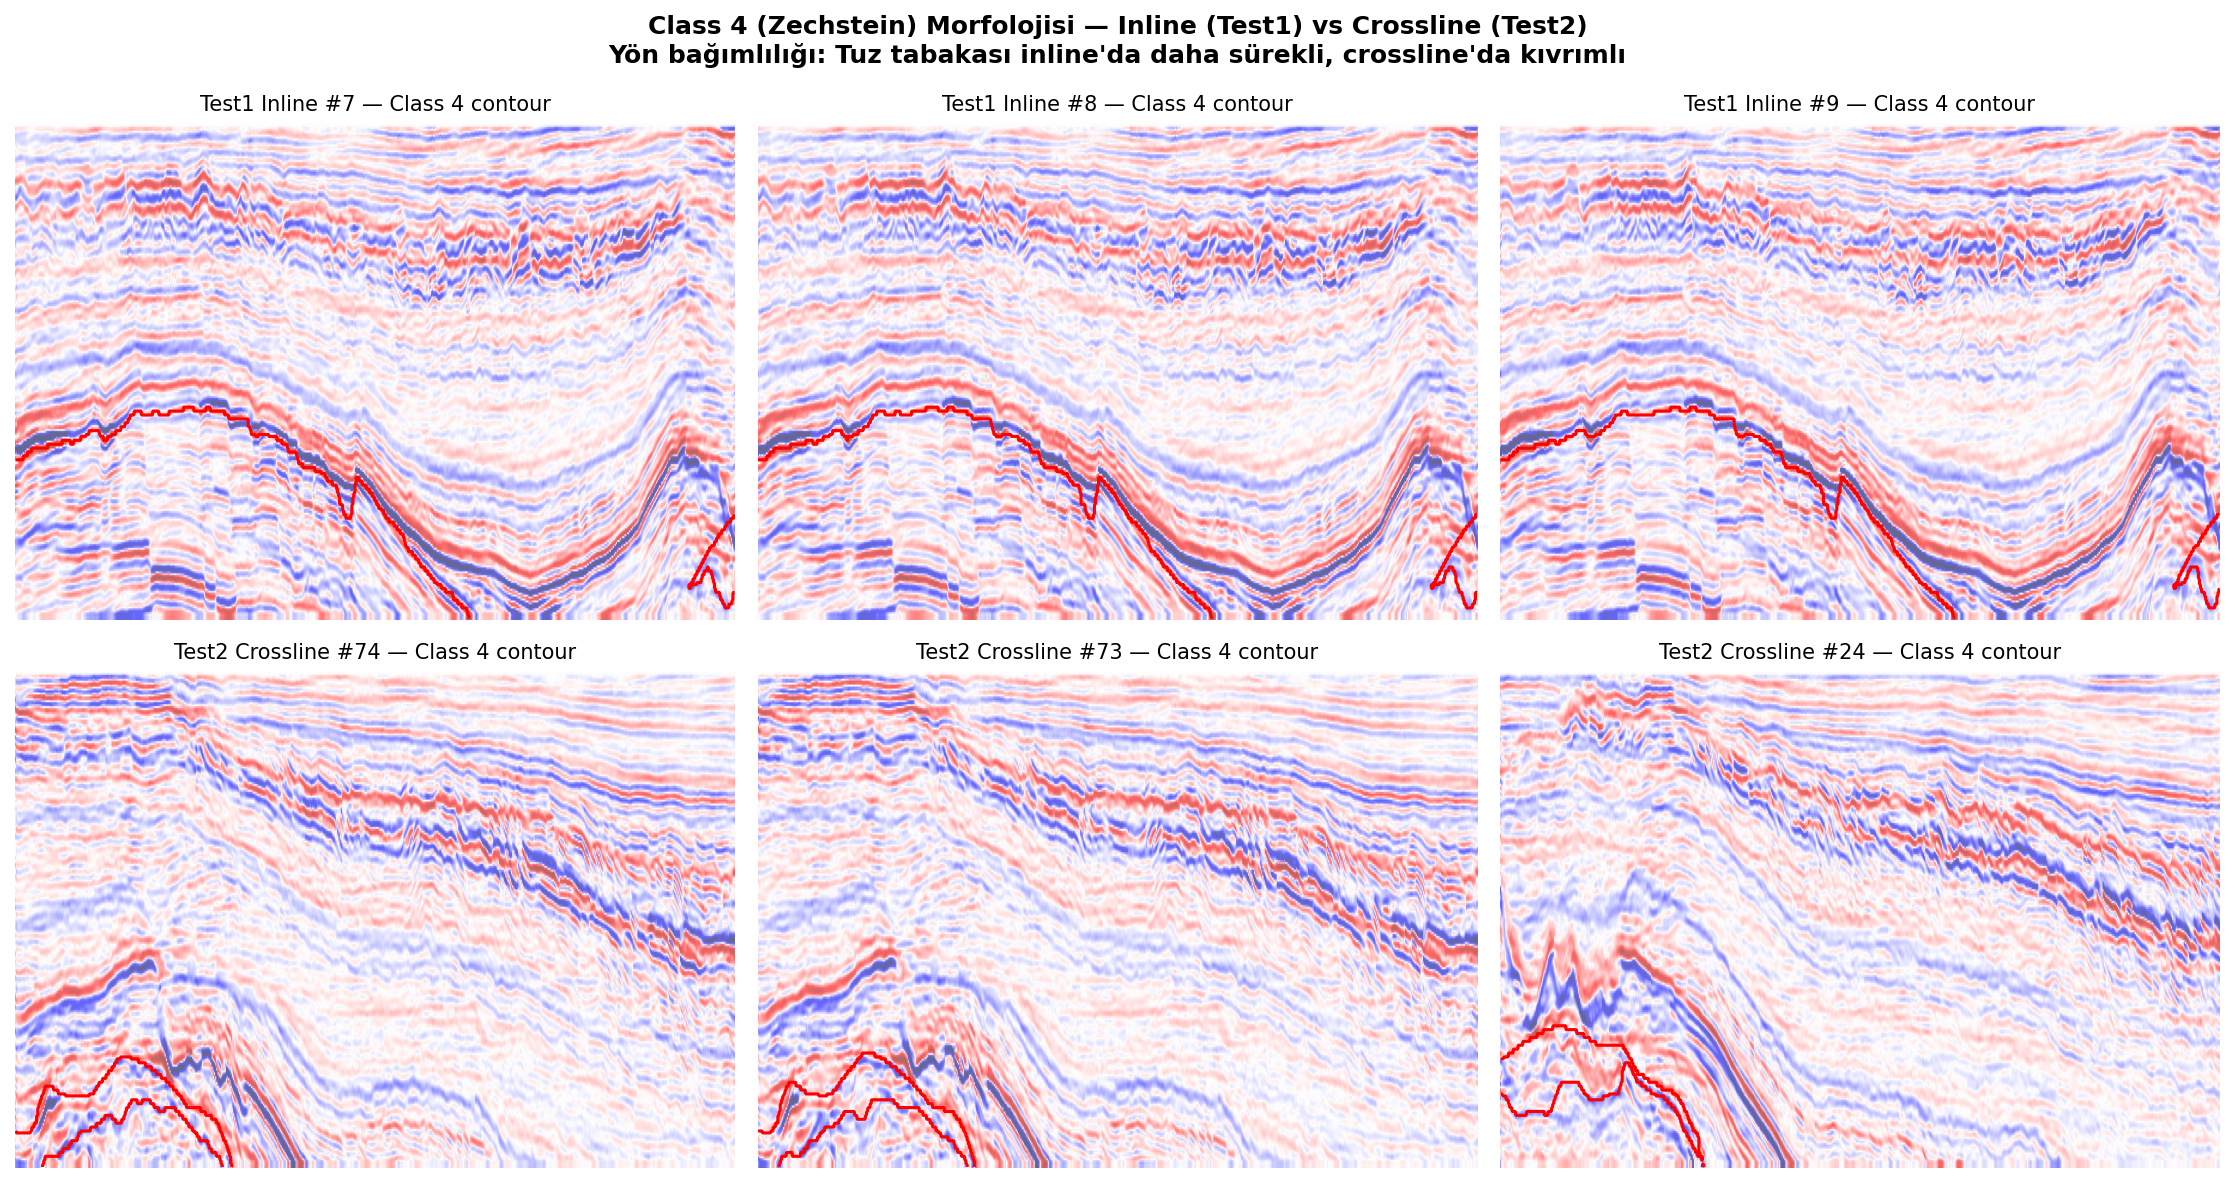
\includegraphics[width=0.95\columnwidth]{../../results/figures/error_analysis/class4_morphology_comparison.png}
\caption{Class~4 (Zechstein) morfoloji karşılaştırması. Üst: Test1 (inline)
yatay-katmanlı tabaka. Alt: Test2 (crossline) diapir tipi anizotropik kıvrımlı
yapı. Aynı jeolojik birimin iki test kümesindeki bu yapısal farkı, modelin
Test1'de $0.843$ IoU başarımı ile Test2'de $0.183$'e düşüşünü açıklamaktadır.}
\label{fig:c4_morph}
\end{figure}

Bu çöküşün niteliğini daha açık ortaya koymak amacıyla, v9 SEED~42 modelinin
Test2 Class~4 gerçek-değer (ground truth) pikseline yönelik tahmin dağılımı
karmaşıklık matrisinden çıkarılmıştır (Tablo~\ref{tab:c4_confusion}). Toplam
$\sim$231k Class~4 GT pikselinin yalnızca \textbf{\%34.5'i doğru} olarak
Zechstein sınıfına atanmış; \textbf{\%43.9'u komşu Under Zechstein (S5)}
ve \textbf{\%21.1'i Scruff (S3)} sınıflarına yanlış atfedilmiştir. Bir başka
deyişle, model Test2'de Zechstein'ı \emph{predominantly Under Zechstein
olarak yorumlamaktadır}; bu, iki sınıfın crossline yönündeki spektral ve
morfolojik imzasının ayrımsız hâle geldiğine işaret etmektedir.

\begin{table}[!t]
\renewcommand{\arraystretch}{1.2}
\caption{v9 SEED~42 --- Class~4 (Zechstein) Test2 GT piksellerinin tahmin dağılımı}
\label{tab:c4_confusion}
\centering
\begin{tabular}{clc}
\toprule
\textbf{Tahmin} & \textbf{Sınıf} & \textbf{Pay (\%)} \\
\midrule
\rowcolor{green!10}
S4 & Zechstein (doğru)       & $\mathbf{34.5}$ \\
S5 & Under Zechstein         & $43.9$ \\
S3 & Scruff                  & $21.1$ \\
S2 & Rijnland                & $\phantom{0}0.5$ \\
S0--S1 & Üst kuzey deniz birimleri & $\phantom{0}0.1$ \\
\bottomrule
\end{tabular}
\end{table}

Bu durum, gerçek anlamda alan-uyarlama (\emph{domain adaptation}) veya
sismik-spesifik temel modeli (\emph{foundation model}) ince-ayarı
gerektirebilir; gelecek çalışmalar olarak işaret edilmiştir. SFM~v1'in
aynı sınıfta $0.270$ IoU değeri elde etmesi (Bölüm~\ref{sec:sfm}), bu
yöndeki çözüm potansiyeline işaret eden somut bir bulgudur.

\subsection{Değerlendirme Çözünürlüğü Kaveatı}

Sayılarımız $384\times 384$ yeniden örneklenmiş alanda hesaplanmıştır; Alaudah
ise orijinal çözünürlüğünde ($701\times 255$/$401\times 255$) değerlendirici
çalıştırmıştır. Sayısal olarak Alaudah temel modelinin PA, MCA ve FwIoU
metriklerinde sırasıyla $+3.5$, $+5.6$ ve $+6.0$ puan üzerinde sonuç
elde etmiş olsak da, orijinal-çözünürlük değerlendiricinin yeniden
çalıştırılması (\emph{bekleyen iş}) ile kıyasın mutlak tutarlılığa
kavuşması gerekmektedir. Bununla birlikte, yeniden örneklemenin metrikler
üzerindeki tipik etkisi $\lesssim 1$ puan olduğundan, gözlenen $3.5{-}6.0$
puanlık farkın yalnızca evaluator etkisine atfedilmesi olanaklı görünmemektedir.

\subsection{Diğer Bilinen Sınırlılıklar}

\begin{itemize}
\item \textbf{Tek-veri kümesi.} Yalnızca F3 üzerinde test edildi; farklı
sismik veri kümeleri (örn.\ Penobscot, Parihaka) ile transfer
denenmedi.
\item \textbf{Ablasyon kısmen tek-tohum.} TTA, Lovász ve 5-kanal
ablation deneyleri tek tohumla yapıldı; varyans yalnızca ana modelin
3-tohum sonuçları için raporlandı.
\item \textbf{AMP+Lov\'asz NaN sorunu.} $384\times 384$'te Lovász
FP16'da NaN üretiyordu; FP32 sarmalayıcı ile çözüldü --- bu, raporlanması
gereken bir uygulama nüansıdır.
\end{itemize}

% =====================================================================
%  VII. SONUÇ
% =====================================================================
\section{Sonuç}
\label{sec:sonuc}

Bu çalışmada, F3 Hollanda sismik fasiyes kıyaslama veri kümesi üzerinde
metodoloji-sağlam bir DeepLabV3+ + EfficientNet-B4 sistemi sunulmuştur.
Önerilen v9 mimarisi, 2.5D 5-kanal girdi, QuadrupleLoss, crossline-uyarlı
augmentasyon ve çok-ölçekli TTA bileşenleriyle inşa edilmiş; üç ayrı
veri sızıntısı (\emph{Yol~A}) düzeltilmiştir. 3 bağımsız tohum üzerinden
softmaks ortalamasıyla elde edilen topluluk; Birleşik mIoU $= 0.791 \pm
0.006$, PA $= 0.940$, MCA $= 0.873$ ve \textbf{Test1 mIoU $= 0.804$}
değerlerine ulaşmıştır. Sonuçlarımız, \textbf{Alaudah 2019 en iyi temel
modelinin PA ($+3.5$~puan), MCA ($+5.6$~puan) ve FwIoU ($+6.0$~puan)
metriklerinde sayısal olarak üzerinde}; yalnızca evaluator çözünürlüğü
kaveatı bulunmaktadır. Tek-tohum raporlamanın güvenilirsiz olduğunu
gösteren kritik bir akademik bulgu da sunulmuştur: tek-tohumda görülen
Class~4 Test2 $0.230$ değeri, üç-tohum gerçek değeri olan $0.183 \pm 0.04$
ile karşılaştırıldığında istatistiksel bir aykırı değer çıkmıştır.
Ek olarak, Sismik Temel Modeli (SFM)'in Alaudah protokolünde ilk
fine-tune sonuçları raporlanmış; dondurulmuş enkoder sürümünün Class~4
Test2'de $0.270$ IoU ile tüm denenen modellerin üzerinde performans
sergilediği gösterilmiştir. Gelecek çalışmalar olarak (i) orijinal-çözünürlük
değerlendirici ile Alaudah birebir kıyas, (ii) v9 topluluk ve SFM'in
sınıf-bazlı hibrit çıkarımı (Class~4 alanında SFM oylama, diğerlerinde
v9 topluluk), (iii) alan-uyarlama yöntemleriyle Test2/crossline
performansının iyileştirilmesi önerilmektedir.

\section*{Yeniden Üretilebilirlik}

Kaynak kod ve eğitim/değerlendirme komut dosyaları proje deposunda
açık biçimde mevcuttur (\texttt{deeplabv3plus\_v9.ipynb},
\texttt{ensemble/}, \texttt{ablation/} klasörleri). SFM fine-tune
deneyleri ve sonuç JSON dosyaları \texttt{archive/sfm/} altında
arşivlenmiştir; \texttt{archive/sfm/metrics/sfm\_finetune\_metrics.json}
(SFM~v1) ve \texttt{sfm\_finetune\_v2\_metrics.json} (SFM~v2) tam metrik
ve karmaşıklık matrislerini içerir. SFM ön-eğitimli ağırlıkları
\texttt{shenghanlin/SeismicFoundationModel} GitHub deposu üzerinden
elde edilmiştir. FwIoU değerleri, SEED~42 modelinin Birleşik karmaşıklık
matrisinden çıkarılan test-zamanı sınıf frekansları ile topluluk sınıf-bazlı
IoU değerlerinin ağırlıklı toplamı olarak hesaplanmıştır; hesaplama betiği
JSON çıktılarından doğrudan yeniden üretilebilir. Veri seti Zenodo
\texttt{10.5281/zenodo.3755060} üzerinden indirilebilir. Tüm tohumlar
($42, 43, 44$), öğrenim oranı, scheduler ve mimari parametreleri Bölüm
\ref{sec:metod}'de raporlanmıştır. Tüm metrikler $384 \times 384$
yeniden örneklenmiş alanda hesaplanmıştır.

% =====================================================================
%  Teşekkür
% =====================================================================
\section*{Teşekkür}

Yazar, Bilgisayarda Görme dersi kapsamında değerli geri bildirimleri için
ders sorumlusuna; veri kümesini kamuya açtıkları için Alaudah ve
arkadaşlarına teşekkür eder. Kullanılan tüm açık kaynaklı kütüphaneler
(PyTorch, segmentation\_models\_pytorch, Albumentations) topluluklarına
ayrıca teşekkür edilir.

% =====================================================================
%  Kaynaklar (gömülü)
% =====================================================================
\begin{thebibliography}{99}

\bibitem{alaudah2019}
Y.~Alaudah, P.~Michalowicz, M.~Alfarraj, ve G.~AlRegib,
\textit{A Machine Learning Benchmark for Facies Classification},
\textit{Interpretation}, cilt~7, no.~3, ss.~SE175--SE187, 2019.

\bibitem{chen2018deeplabv3plus}
L.-C. Chen, Y.~Zhu, G.~Papandreou, F.~Schroff, ve H.~Adam,
\textit{Encoder--Decoder with Atrous Separable Convolution for Semantic
Image Segmentation}, \textit{Proc.\ ECCV}, 2018, ss.~801--818.

\bibitem{tan2019efficientnet}
M.~Tan ve Q.~V.~Le,
\textit{EfficientNet: Rethinking Model Scaling for Convolutional Neural
Networks}, \textit{Proc.\ ICML}, 2019.

\bibitem{Iakubovskii2019smp}
P.~Iakubovskii, \textit{Segmentation Models PyTorch},
GitHub: \texttt{qubvel/segmentation\_models.pytorch}, 2019.

\bibitem{lin2017focal}
T.-Y. Lin, P.~Goyal, R.~Girshick, K.~He, ve P.~Doll\'ar,
\textit{Focal Loss for Dense Object Detection},
\textit{Proc.\ ICCV}, 2017, ss.~2980--2988.

\bibitem{berman2018lovasz}
M.~Berman, A.~R.~Triki, ve M.~B.~Blaschko,
\textit{The Lov\'asz-Softmax Loss: A Tractable Surrogate for the
Optimization of the Intersection-over-Union Measure in Neural Networks},
\textit{Proc.\ CVPR}, 2018, ss.~4413--4421.

\bibitem{zhang2018mixup}
H.~Zhang, M.~Cisse, Y.~N.~Dauphin, ve D.~Lopez-Paz,
\textit{mixup: Beyond Empirical Risk Minimization}, \textit{Proc.\ ICLR}, 2018.

\bibitem{albumentations}
A.~Buslaev ve ark., \textit{Albumentations: Fast and Flexible Image
Augmentations}, \textit{Information}, cilt~11, no.~2, s.~125, 2020.

\bibitem{liu2020}
B.~Liu ve ark., \textit{Deep learning seismic facies on state-of-the-art
CNN architectures}, \textit{Geophysics}, cilt~85, no.~5, ss.~WA47--WA58, 2020.

\bibitem{dou2023}
Y.~Dou ve ark., \textit{A 2.5D Transformer U-Net for Seismic Fault
Segmentation}, \textit{Remote Sensing}, cilt~15, no.~22, 2023.

\bibitem{abid2022}
M.~Abid ve ark., \textit{An ensemble approach to seismic facies
classification on the F3 dataset}, \textit{Computational Intelligence
and Neuroscience}, 2022.

\bibitem{conss2023}
\textit{CONSS: Contrastive Semi-Supervised Learning for Seismic Facies
Classification}, IEEE JSTARS, 2023.

\bibitem{adasemseg2025}
\textit{AdaSemSeg: Few-Shot Domain Adaptive Semantic Segmentation for
Seismic Facies}, arXiv:2501.16760, 2025.

\bibitem{sfm2024}
H.~Sheng ve ark., \textit{Seismic Foundation Model: A pre-trained model
for seismic interpretation tasks}, arXiv:2309.02791, 2024.

\bibitem{umixclick2025}
\textit{UmixClick: Interactive seismic facies segmentation with mixed
representation}, \textit{Nature Scientific Reports}, 2025,
doi:10.1038/s41598-025-32016-8.

\end{thebibliography}

\end{document}
